\thispagestyle{fancy}
	
	\vspace{-2em} % Adjust vertical space as needed
	\begin{center}



\addcontentsline{toc}{subsection}{Message of the Dean, Faculty of Education}    
\subsection*{\textsc{Message of the Dean, Faculty of Education}}
	\end{center}

   
    
    \begin{wrapfigure}{l}{0.3\textwidth}
		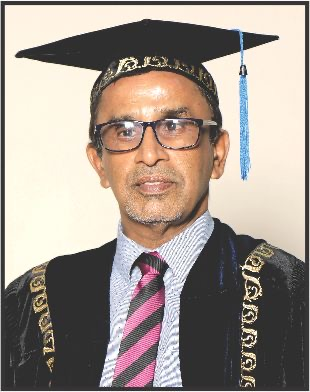
\includegraphics[width=0.3\textwidth]{Images/DeanFE.jpeg}
	\end{wrapfigure}
	\vspace{2em} % Adjust vertical space as needed




	
	
	
	
	It is a great pleasure to issue this message on the occasion of the International Research Symposium (IRS), 2024 of the University of Vocational Technology. The Symposium is an annual event in the academic calendar of the University and has been a great success in the last several years.
    
The University has continued to promote conducive environment for increased generation of quality research while enabling mentorship of early researchers through research methodology and data analysis capacity development. We believe that dissemination of knowledge and providing    exposure to staff and students to engage in research is a part of our responsibility. It is a great opportunity for them to improve their analytical skills and interact with a wider community.

This annual symposium will provide an excellent platform for students and faculty members of the University, other public and private universities and research institutions to show-case their research productivity and promise for the future new knowledge generation.

Finally, I would like to thank the organizing committee and others who have worked hard to contribute to the success of this symposium.
 


	\vspace{1cm}
	\noindent
	Dr.Sunil Kularatne\\
Dean\\
Faculty of Education
	\newpage
	